\section{Reducing the Number of Calculations}
\subsection{The problem}
As we've seen in the introduction, Newton's equation
\begin{equation}
\frac{d^2\vec{r}_i}{dt^2}=G\sum_{j\neq i}m_j\frac{\vec{r_j}-\vec{r_i}}{|\vec{r_j}-\vec{r_i}|^3}
\label{Newton G}
\end{equation}
applies on every object in our solar system. Thus, for every of the $N$ objects in the system, the pairwise forces of the other $N-1$ objects need be calculated. This means that for every time step $\Delta t$, the number of calculations equals $N(N-1)$. Therefore the brute force algorithm has complexity $\orde{N^2}$. For 1000 objects and 12000 time steps, one need to perform at most $1000^2\cdot 12000 = 12000000000$ (12 billion) calculations -- collisions excluded. This is insufficient for most computers.
\subsection{The Barnes-Hut algorithm: a partial solution}
To reduce the amount of calculations on equation \ref{Newton G}, we make use of the \textit{Barnes-Hut Algorithm}.\cite{barneshut} The general idea is to treat objects that are 'sufficiently near each other' in comparison to their distance from the considered object, as one.\\
\textbf{Algorithm.}
\begin{enumerate}
\item First, consider the whole space, which must have a boundary, so we take the 'whole space' to be the hypercube that encapsulates all objects to consider (in our case, we use the center of impulse as the center of the space). Create a node, which will become the root of the Barnes-Hut tree, that contains the total mass and center of mass of all objects. If the space contains only one object (or no objects), we do nothing; otherwise, cut the hypercube in half in every dimension, and for every such created subspace, create a child of the root that represents that subspace, including the total mass and center of mass of the objects in that subspace.
\item For every such created subspace, recursively check whether the subspace contains zero, one or more than one objects. If it contains zero or one object, do nothing; otherwise, cut the space in subspaces accordingly and create child nodes for every subspace containing the center of mass and total mass of the objects in that subspace.
\item When every node that has no children contains either zero or one object, the Barnes-Hut tree is completed.
\item For every object $a$, do the following.
\begin{enumerate}
\item Start at the root of the current Barnes-Hut tree.
\item For the current node, if the node represents zero objects, skip that node. If the node represents one object, calculate the force that object excerts on $a$. If the node represents more than one object (and thus is an internal node), calculate the ratio $\frac{s}{d}$, where $s$ is the length of the space - that is, the distance in one dimension from one side to the other - represented by the node (i.e the whole space has length, say, $L$, then the root's children have length $L/2$, etc.), and $d$ is the distance between the center of mass of the node and $a$.
\item Choose a certain parameter $\theta \in \R_{>0}$. If $\frac{s}{d}<\theta$, then treat the node as a single object with mass and center of mass of that node. Otherwise, recursively repeat (b) and (c) for the node's children.
\end{enumerate}
\end{enumerate}
\newpage
\textbf{Example.} Consider the following map, which is a more detailed example than in \cite{barneshut}.
\begin{figure}[ht]
\centering
\begin{subfigure}{0.35\textwidth}
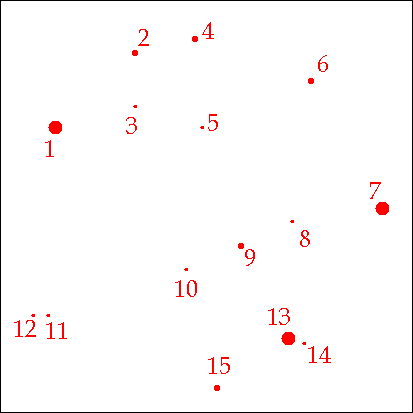
\includegraphics[width=\textwidth]{barneshut_map.png}
\caption{An example of a map with objects. The boundary of the map is already given.}
\end{subfigure}\hspace{1cm}
\begin{subfigure}{0.35\textwidth}
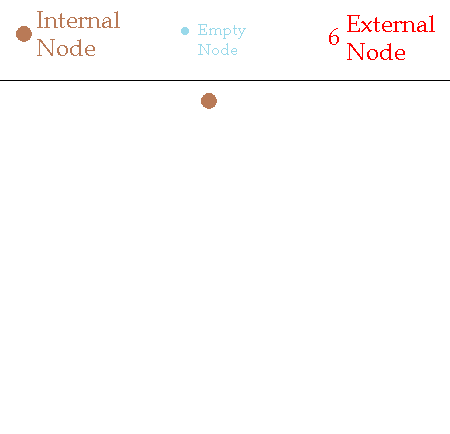
\includegraphics[width=\textwidth]{barneshut_tree_root.png}
\caption{The current tree, containing only the root.}
\end{subfigure}
\caption{The starting situation.}
\end{figure}
Splitting the space and filling the tree, we get the following result.
\begin{figure}[ht]
\centering
\begin{subfigure}{0.35\textwidth}
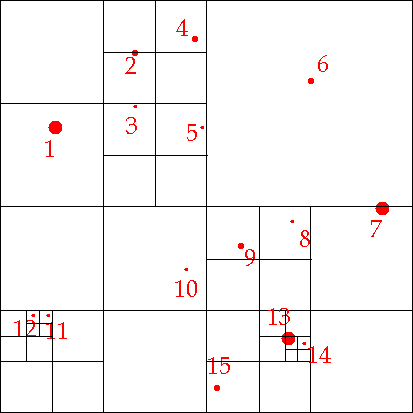
\includegraphics[width=\textwidth]{barneshut_map_devided.png}
\caption{An example of a map with objects. Now the space is devided in subspaces such that every object has it's own subspace.}
\end{subfigure}\hspace{1cm}
\begin{subfigure}{0.35\textwidth}
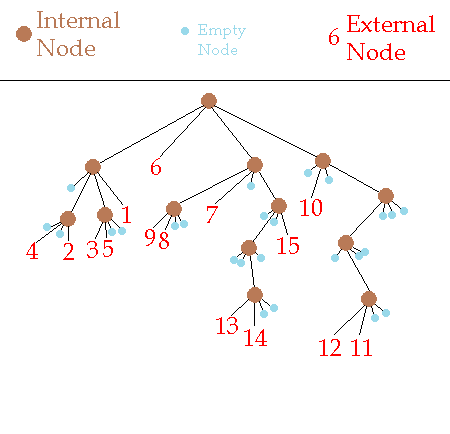
\includegraphics[width=\textwidth]{barneshut_tree.png}
\caption{The final tree.}
\end{subfigure}
\caption{The final situation.}
\end{figure}
Note that we build the tree, starting from the northwest subspace of a node and proceeding clockwise.\\

Now let's say we want to calculate the net force on object 15, and we use $\theta = \frac{1}{3}$. In this case, both the root and it's children do not satisfy $\frac{s}{d} < \frac{1}{3}$, so since 6 is an external node, we add the pairwise force between 6 and 15 to 15's net force. Moving one level down, any node with center of mass outside the green zone showed below can be treated as one object.
\begin{figure}[ht]
\centering
\begin{subfigure}{0.24\textwidth}
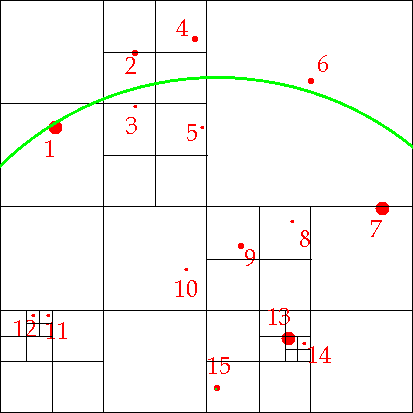
\includegraphics[width=\textwidth]{barneshut_map_green_2.png}
\caption{The green zone indicates which internal nodes can be treated as one (outside), and which can't (inside).}
\end{subfigure}\hspace{1cm}
\begin{subfigure}{0.24\textwidth}
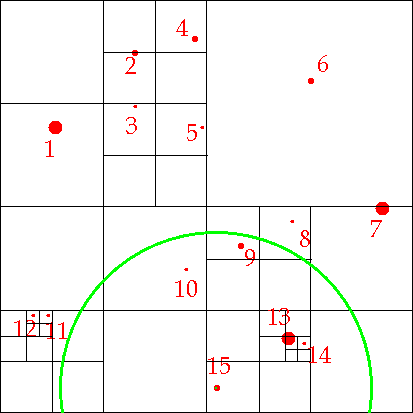
\includegraphics[width=\textwidth]{barneshut_map_green_3.png}
\caption{The green zone indicates which internal nodes can be treated as one (outside), and which can't (inside).}
\end{subfigure}\hspace{1cm}
\begin{subfigure}{0.24\textwidth}
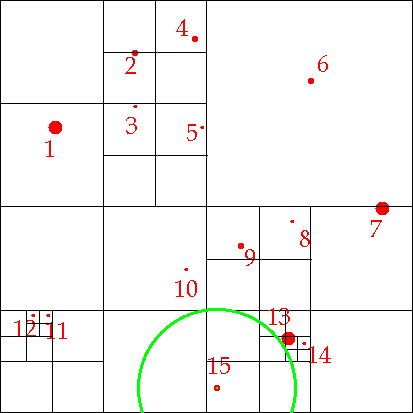
\includegraphics[width=\textwidth]{barneshut_map_green_4.png}
\caption{The green zone indicates which internal nodes can be treated as one (outside), and which can't (inside).}
\end{subfigure}\hspace{1cm}
\begin{subfigure}{0.24\textwidth}
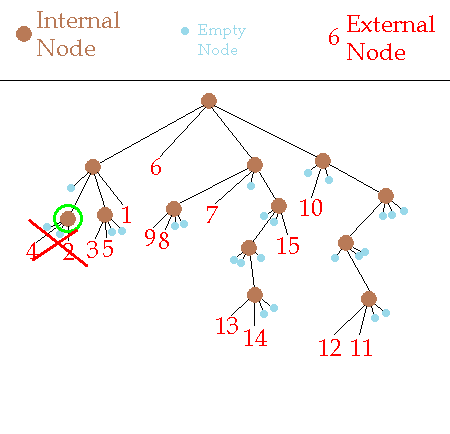
\includegraphics[width=\textwidth]{barneshut_tree_node_4_2.png}
\caption{The green node can be treated as a single object.}
\end{subfigure}\hspace{1cm}
\begin{subfigure}{0.24\textwidth}
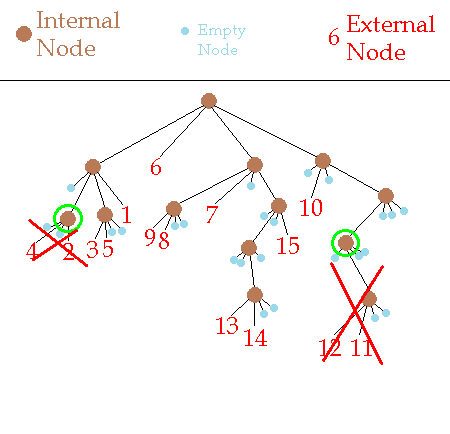
\includegraphics[width=\textwidth]{barneshut_tree_node_lvl3.png}
\caption{The green node can be treated as a single object.}
\end{subfigure}\hspace{1cm}
\begin{subfigure}{0.24\textwidth}
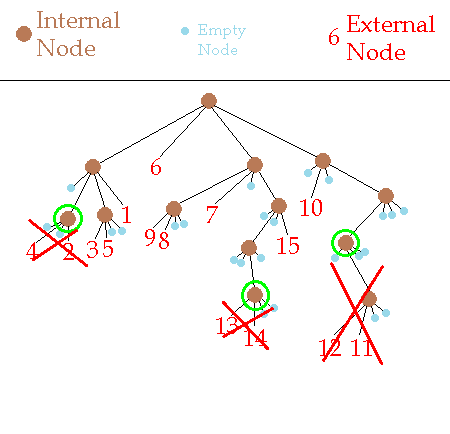
\includegraphics[width=\textwidth]{barneshut_tree_node_lvl4.png}
\caption{The green node can be treated as a single object.}
\end{subfigure}
\caption{Check which nodes can be treated as one object, at different levels (root is level 0, root's children are level 1, etc.): left corresponds to level 2, center to level 3, right to level 4.}
\end{figure}
The figure indicates that we must calculate the pairwise forces of object 15 with objects 1,3,5,6,7,8,9,10, but we can group objects 2 and 4, 11 and 12, and 13 and 14 to be treated as one object to calculate the force on object 15.
The computer uses the algorithm recursively, so it will first check the first child of the root, it's children, etc, before moving on to the root's second child.

\subsection{Analysis: complexity}
The strength of the Barnes-Hut algorithm is that the tree is built only once per time step. Thus, for every object one just has to 'walk through the tree' without having to create it. We will make this point more specific.
\subsubsection*{Building the tree} Using the same terminology as the previous example, we can note that, for every level of the tree, there are at most $N$ objects represented by the nodes of that level. For a node representing $k$ objects, calculating the center of mass takes $2k$ elementary operations ($k$ multiplications and $k$ additions), and the calculation of the total mass takes $k$ additions. So in total there are $3k$ elementary operations. Therefore, for every level, there are at most $3N$ elementary operations to do.\\
Now looking at the number of levels, we can give a lower bound but unfortunately no upper bound. For a $D$-dimensional space, a node has ideally $2^D$ children with an equal amount of objects. In this case there will be $\ceiling{^{2^D} \log(N)} = \ceiling{\frac{^2\log(N)}{D}}$ levels, which is the lower bound.\\
Unfortunately, there can't be said anything about the upper bound; simply take one object to be randomly far away from two others. In this case, the tree just goes down and every node contains exactly the same information as it's parent, except for the last one, which has two external children. Fortunately, according to our simulations, the vast majority of the time, the number of levels isn't much greater than the lower bound. Assuming the lower bound, we have a complexity for building the tree of $\orde{N\log(N)}$.
\subsubsection*{Number of calculations, given a tree} Let $i$ be a given object, and $D$ the dimension of our space. As we have seen in the example, we can draw a hypersphere outside which a node can be treated as a single object. Since this hypersphere changes in size according to the size of the piece of space represented by the node, there's a constant maximum $M_\theta$ of nodes of a certain level that fall \textit{inside} the sphere. The other $M_\theta(2^D-1)$ fall outside and can be calculated - if not already done before at a previous level. So at the previous level there were $M_\theta$ or less nodes that could not be simplified. At the current level, $M_\theta$ or less of those cannot be simplified and the other $M_\theta(2^D-1)$ can. This applies for every level that satisfies $M_\theta \leq 2^{\text{level}}$. Thus, for every level the number of calculations is at most
\[
M_\theta (2^D-1) := c(\theta)
\]
We have noted earlier that there is no upper bound for the number of levels. However, with the number of levels approximately $\orde{\log(N)}$, the total number of calculations for object $i$ should be $\orde{\log(N)}$. Therefore the total number of calculations on one time step is $\orde{N\log(N)}$, but again this is on average, not worst case.
\subsubsection*{Conclusion}
\textbf{In conclusion, we can not state the Barnes-Hut algorithm always gives a reduction on the number of calculations, but on average, the number of calculations reduces from $\orde{N^2}$ to $\orde{N\log(N)}$.}
\subsection{Analysis: Precision and the Size of the Error}
As one can expect, the precision of the Barnes-Hut algorithm is total dependent on it's sole parameter $\theta$. We will first make a few remarks.
\begin{enumerate}
\item Let $D$ be the dimension of the considered space, and suppose $\theta \geq \frac{1}{\sqrt{D}}$. Consider the condition $\frac{s}{d} < \theta$. This implies
\[
s < d\theta \geq \frac{d}{\sqrt{D}}
\]
Thus, $s$ might be greater than $\frac{d}{\sqrt{D}}$. Noting that the distance between two objects in the same subspace is at most $\sqrt{Ds^2} = s\sqrt{D}$, which might imply $s\geq d$. So, it might be that the algorithm considers an object in the same subspace as to be sufficient far away. In this case the algorithm lets an object excert force on itself -- strictly forbidden. So $\theta$ must be smaller than $\frac{1}{\sqrt{D}}$. We will see later that strictly smaller applies.
\item Note that the calculated force is always less or equal the actual force. This is because the center of mass is used -- but the closer objects excert more force than the farther objects.
\item Consider a subspace represented by a node, that contains two objects. Let $d_1$ be the distance from the considered object to the first object, and let $d_2$ be defined similarly. In addition, let $m_1$ be the mass of the first object and $m_2$ the mass of the second object. Consider the error in the force calculated
\[
E(m_1,m_2,d_1,d_2) = \frac{m_1}{d_1^2}+\frac{m_2}{d_2^2}-\frac{m}{d^2}
\]
where $m = m_1+m_2$ and $d = \frac{m_1d_1+m_2d_2}{m}$ is the center of mass.\\
We will prove that the error reaches no maximum in terms of $\Delta d$. Suppose
\[
\begin{array}{cc}
m_2 = cm_1, c\in \R_{>0}, & d_2-d_1 = \Delta d
\end{array}
\]
We can now express $m_1,m_2,d_1,d_2$ in terms of $m,d,c,\Delta d$: one can easily check that
\begin{align*}
m_1 &= \frac{1}{1+c}m\\
m_2 &= \frac{c}{1+c}m\\
d_1 &= d-\frac{m_2}{m}\Delta d = d-\frac{c}{1+c}\Delta d\\
d_2 &= d+\frac{m_1}{m}\Delta d = d+\frac{1}{1+c}\Delta d
\end{align*}
Now the error reduces to
\[
E = \frac{m\frac{1}{1+c}}{(d-\frac{c}{1+c}\Delta d)^2}+\frac{m\frac{c}{1+c}}{(d+\frac{1}{1+c}\Delta d)^2}-\frac{m}{d^2}
\]
To determine the extrema of this error with respect to $\Delta d$, we take the derivative to $\Delta d$.
\begin{align*}
\frac{\partial E}{\partial \Delta d} &= \frac{m}{1+c}\left(d-\frac{c}{1+c}\Delta d\right)^{-3}2\frac{c}{1+c}+\frac{mc}{1+c}\left(d+\frac{1}{1+c}\Delta d\right)^{-3}\left(-2\frac{1}{1+c}\right)\\
&= 2\frac{mc}{(1+c)^2}\left(\left(d-\frac{c}{1+c}\Delta d\right)^{-3}-\left(d+\frac{1}{1+c}\Delta d\right)^{-3}\right)
\end{align*}
Setting this derivative equal to zero reduces to
\[
\left(d-\frac{c}{1+c}\Delta d\right)^3 = \left(d+\frac{1}{1+c}\Delta d\right)^3
\]

\end{enumerate}